\documentclass{beamer}
\title{Conception d'un processeur pipeliné avec \textit{forwarding}}
\subtitle{Architecture des systèmes numériques}
\author{Arthur \textsc{Jacquin}, Martin \textsc{François}}
\institute{\textsc{CentraleSupélec - Université Paris-Saclay}}


% PACKAGES, CONFIGURATION

% Language and encoding
\usepackage[utf8]{inputenc}
\usepackage[T1]{fontenc}
\usepackage[french]{babel}

% Colors
\usepackage{xcolor}
\definecolor{darkseahorseblue}{RGB}{153,153,215}
\definecolor{blue}{RGB}{0,68,204}
\definecolor{green}{RGB}{0,153,0}

% Figures
\usepackage{caption}
\DeclareCaptionFont{captioncolor}{\color{darkseahorseblue}}
\captionsetup{labelfont={captioncolor}}
\DeclareCaptionLabelSeparator{sep}{ : }
\captionsetup{labelsep=sep}

% Code
\usepackage{listings}
\lstdefinestyle{simple}{
    extendedchars=true,
    basicstyle=\ttfamily\tiny,
    backgroundcolor=,
    commentstyle=\color{green},
    keywordstyle=\color{blue},
    numberstyle=\ttfamily\color[rgb]{0.5,0.5,0.5},
    breakatwhitespace=false,
    breaklines=true,
    captionpos=b,
    keepspaces=true,
    numbers=left,
    numbersep=7pt,
    showspaces=false,
    showstringspaces=false,
    showtabs=false,
    tabsize=4,
    columns=fixed
}
\lstset{style=simple}

% Tables
\usepackage{booktabs}

% Links
\usepackage{hyperref}

% Math
\usefonttheme[onlymath]{serif}

% Theme
\usetheme{default}
\usecolortheme{seahorse}
\setbeamertemplate{navigation symbols}{}
\setbeamertemplate{footline}[frame number]
\setbeamertemplate{itemize items}{\color{darkseahorseblue}$\bullet$}
\setbeamertemplate{caption}[numbered]


% CONTENT

\begin{document}

% Title page
\frame{\titlepage}

% Sommaire
\begin{frame}
\frametitle{Sommaire}
\begin{itemize}
\item ISA
    \begin{itemize}
    \item Formats
    \item Codes des instructions
    \item Sauts (in)conditionnels
    \end{itemize}
\item Pipeline
\item Architecture générale
\item Décodeur
\item Assembleur
\item Test
    \begin{itemize}
    \item Protocole
    \item Programme
    \item Résultats
    \end{itemize}
\end{itemize}
\end{frame}

% ISA - Formats
\begin{frame}
\frametitle{ISA - Formats}
\begin{itemize}
\item 16 registres de 16 bits
\item code d'instruction en deux parties : \texttt{op}, commun à tous les
    formats, et \texttt{funct}, permettant une plus grande granularité avec les
    instructions manipulant plusieurs opérandes mais inexistant pour celles où
    un immédiat occupe beaucoup de bits.
\end{itemize}
\medskip
\begin{table}[ht]
    \centering
    \begin{tiny}
    \begin{tabular}{cl}
    \toprule
    \texttt{fmt} & Champs (nom et taille) \\
    \midrule
    \texttt{00} & \texttt{fmt[2] op[4] dest[4] src1[4] funct[2] [6] src2[4]} \\
    \texttt{01} & \texttt{fmt[2] op[4] dest[4] src1[4] funct[2] imm[10]} \\
    \texttt{10} & \texttt{fmt[2] op[4] dest[4] imm[16]} \\
    \bottomrule
    \end{tabular}
    \end{tiny}
    \caption{Formats de l'ISA}
    \label{tab:formats}
\end{table}
\begin{table}[ht]
    \centering
    \begin{tiny}
    \begin{tabular}{cc}
    \toprule
    Catégorie & Description \\
    \midrule
    A & nécessite \texttt{funct}, \texttt{fmt} = \texttt{00} ou \texttt{01} \\
    B & nécessite un grand immédiat, \texttt{fmt} = \texttt{10} \\
    C & autres, \texttt{fmt} = \texttt{00} ou \texttt{10} \\
    \bottomrule
    \end{tabular}
    \end{tiny}
    \caption{Catégories d'instructions}
    \label{tab:instructions_types}
\end{table}
\end{frame}

% ISA - Codes des instructions
\begin{frame}
\frametitle{ISA - Codes des instructions}
\begin{table}[ht]
    \centering
    \begin{tiny}
    \begin{tabular}{ccccl}
    \toprule
    \texttt{op} & Catégorie & \texttt{funct} & Mnémonique & Commentaire \\
    \midrule
    \texttt{0000} & A & & & Opérations bit à bit \\
    & & \texttt{00} & \texttt{not} & \\
    & & \texttt{01} & \texttt{and} & \\
    & & \texttt{10} & \texttt{or} & \\
    & & \texttt{11} & \texttt{xor} & \\
    \texttt{0001} & A & & & Décalages de bits \\
    & & \texttt{00} & \texttt{rls} & \\
    & & \texttt{01} & \texttt{lls} & \\
    \texttt{0010} & A & & & Opérations arithmétiques \\
    & & \texttt{00} & \texttt{add} & \\
    & & \texttt{01} & \texttt{sub} & \\
    & & \texttt{10} & \texttt{mul} & \\
    \texttt{0011} & A & & & Manipulation de la pile \\
    & & \texttt{00} & \texttt{pop} & \\
    & & \texttt{01} & \texttt{read} & \\
    & & \texttt{10} & \texttt{push} & \\
    \texttt{0100} & B & & \texttt{jmp} & \\
    \texttt{0101} & C & & \texttt{mov} & \\
    \texttt{0110} & B & & \texttt{call} & \\
    \texttt{0111} & C & & \texttt{ret} & \\
    \bottomrule
    \end{tabular}
    \end{tiny}
    \caption{Codes des instructions}
    \label{tab:opcodes}
\begin{itemize}
\item Pseudo-instructions : \texttt{inc}, \texttt{dec}, \texttt{beq},
    \texttt{bne}, \texttt{bgt}, \texttt{bge}, \texttt{blt}, \texttt{ble}
\end{itemize}
\end{table}
\end{frame}

% ISA - Sauts (in)conditionnels
\begin{frame}
\frametitle{ISA - Sauts (in)conditionnels}
\begin{itemize}
\item Tous les sauts sont considérés comme conditionnels par le processeur, avec
    une condition tautologique pour le saut "inconditionnel" \texttt{jmp}
    \begin{itemize}
    \item permet de n'occuper qu'un code dans l'ISA (\texttt{op = 0100})
    \end{itemize}
\item Conditions encodés avec un masque (tableau d'exigence) dans le champ
    \texttt{dest}, par exemple :
    \begin{itemize}
    \item \texttt{0000} $\rightarrow$ aucune exigence $\rightarrow$ saut
        "inconditionnel" \texttt{jmp}
    \item \texttt{0100} $\rightarrow$ exige la comparaison "non égaux"
        $\rightarrow$ saut conditionnel associé à la mnémonique \texttt{bne}
        (\textit{branch non equal})
    \end{itemize}
\item Masques gérés par l'assembleur et non l'utilisateur grâce à l'utilisation
    des pseudo-instructions
\end{itemize}
\end{frame}

% Pipeline
\begin{frame}
\frametitle{Pipeline}
\begin{itemize}
\item plusieurs étapes de traitement $\rightarrow$ les différentes parties du
    processeur n'ont pas besoin d'être synchrones (le synchronisme étant géré
    par les registres tampons séparant les étapes)
    \begin{itemize}
    \item change la syntaxe et les possibilités en VHDL
    \end{itemize}
\item crée des \textit{aléas} :
    \begin{itemize}
    \item de contrôle (incertitude de l'instruction à charger lors d'un saut
        conditionnel)
    \item de données (utilisation d'un registre dont la valeur a été modifiée
        par une instruction précédente depuis sa lecture dans le
        \textit{register file})
    \end{itemize}
\item pour gérer les aléas de contrôle, le décodeur met en pause le programme
    (\textit{stalling}) en remplaçant ses instructions par une instruction sans
    effet (\texttt{or x0, x0, x0})
\item pour gérer les aléas de données, un cache dans l'étape de calcul mémorise
    l'adresse et la valeur du dernier registre calculé (\textit{forwarding})
    \begin{itemize}
    \item si ce même registre est utilisé dans le calcul suivant, la valeur du
        cache remplace celle (obsolète) provenant du \textit{register file}
    \end{itemize}
\end{itemize}
\end{frame}

% Architecture générale
\begin{frame}
\frametitle{Architecture générale}
\begin{figure}
\centering
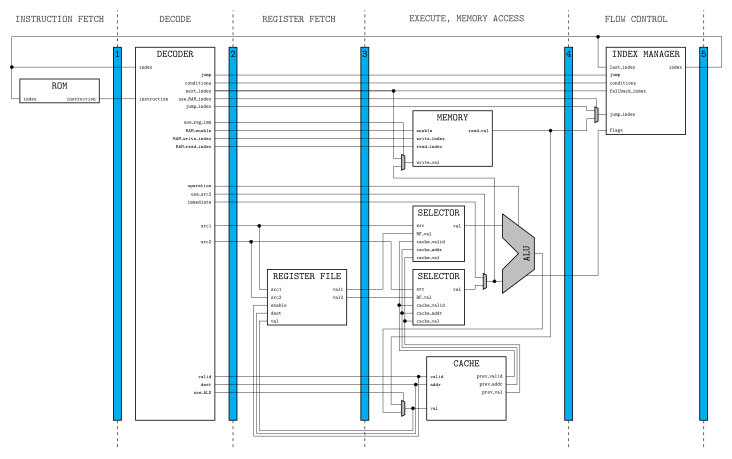
\includegraphics[width=\textwidth]{doc.png}
\caption{Architecture générale du processeur}
\end{figure}
\end{frame}
\begin{frame}
\frametitle{Architecture générale}
\begin{itemize}
\item Les barres bleues symbolisent les registres tampons entre les étapes
\item Pour plus de clarté, certains détails sont omis :
    \begin{itemize}
    \item connexions à l'arbre d'horloge et au signal de réinitialisation
    \item tailles des bus
    \item opérations occasionnelles de redimensionnement des bus
    \end{itemize}
\item Le décodeur utilise le signal interne \texttt{NB\_WAIT} pour savoir
    combien de cycles d'horloge attendre
    \begin{itemize}
    \item Ce signal est modifié par un processus synchrone
    \end{itemize}
\item Le décodeur est le seul composant du processeur prenant en compte le
    signal de réinitialisation, en sautant à l'instruction d'adresse 0
\end{itemize}
\end{frame}

% Décodeur
\begin{frame}[fragile]
\frametitle{Décodeur - 1/3}
\lstinputlisting[language=VHDL, caption=\texttt{decoder.vhd},
    firstline=51, firstnumber=51, lastline=72]{vhdl/decoder.vhd}
\end{frame}
\begin{frame}[fragile]
\frametitle{Décodeur - 2/3}
\lstinputlisting[language=VHDL, caption=\texttt{decoder.vhd},
    firstline=74, firstnumber=74, lastline=83]{vhdl/decoder.vhd}
\end{frame}
\begin{frame}[fragile]
\frametitle{Décodeur - 3/3}
\lstinputlisting[language=VHDL, caption=\texttt{decoder.vhd},
    firstline=85, firstnumber=85, lastline=103]{vhdl/decoder.vhd}
\end{frame}

% Assembleur
\begin{frame}
\frametitle{Assembleur}
\begin{itemize}
\item code binaire peu lisible et manipulable par l'humain $\rightarrow$
    conception d'un assembleur
    \begin{itemize}
    \item programme qui transforme un programme composé de mnémoniques (sous
        forme de fichier textuel facile à manipuler) en code binaire
    \end{itemize}
\item parcourt deux fois le programme :
    \begin{itemize}
    \item analyse syntaxique, formation de la liste des labels
    \item remplacement des labels par leur adresse (\textit{link}), génération
        du code
    \end{itemize}
\item effectue des vérifications :
    \begin{itemize}
    \item validité de la syntaxe
    \item existence et unicité de chaque label utilisé
    \item taille et positivité des immédiats
    \end{itemize}
\end{itemize}
\end{frame}

% Test - Protocole
\begin{frame}
\frametitle{Test - Protocole}
\begin{itemize}
\item Pour tester le processeur, on peut s'assurer que l'exécution de certains
    programmes donne bien les résultats attendus, en étudiant les valeurs de
    certains signaux et registres d'intérêt
\item Pour simuler le fonctionnement du processeur, on utilise un
    \textit{testbench} générant une horloge et un signal de réinitialisation
    actif pendant les premiers cycles d'horloge
\item Ici, on choisit comme test un programme calculant $F_{12}$ (le treizième
    terme de la suite de Fibonacci), car il permet d'utiliser plusieurs
    fonctionnalités :
    \begin{itemize}
    \item copie de valeurs entre plusieurs registres
    \item quelques opérations arithmétiques
    \item utilisation d'immédiats et de registres pour les opérandes
    \item sauts conditionnels et inconditionnels
    \end{itemize}
\end{itemize}
\end{frame}

% Test - Programme
\begin{frame}
\frametitle{Test - Programme}
\begin{columns}
\begin{column}{.5\textwidth}
\lstinputlisting[caption=\texttt{fibo.asb}]{test.asb}
\end{column}
\begin{column}{.5\textwidth}
\lstinputlisting[caption=\texttt{fibo.out}]{out}
\end{column}
\end{columns}
\end{frame}

% Test - Résultats
\begin{frame}
\frametitle{Test - Résultats}
\begin{figure}
\centering
\includegraphics[width=\textwidth]{rapport/figures/simulation.png}
\caption{Résultats de l'exécution de \texttt{fibo.out}}
\end{figure}
\begin{itemize}
\item L'évolution de \texttt{NB\_WAIT}, \texttt{index} et \texttt{ins} semble
    confirmer la bonne gestion des sauts
\item La valeur finale stockée dans \texttt{x1} est $0b10010000 = 144$. Or
    $F_{12} = 144$: on a bien le résultat attendu !
\item Plus de tests (par exemple la pile) sont toutefois nécessaires pour
    garantir le bon fonctionnement du processeur
\end{itemize}
\end{frame}

% Annexes
\begin{frame}
\frametitle{Annexes}
\centering
Toutes les ressources : \url{github.com/arthur-jacquin/cpu}
\end{frame}

\end{document}
